\documentclass{article}

\usepackage{amsmath}
\usepackage{amsthm}
\usepackage{eucal}
\usepackage{amssymb}
\usepackage{color}
\usepackage{tikz}
\usetikzlibrary{shapes,arrows.meta,backgrounds}
\usepackage{etoolbox}
\usepackage{url} % for urls in bibliography
\usepackage[parfill]{parskip} % no paragraph indents, leave blank line
\usepackage{graphicx}
\usepackage{subcaption}
\usepackage{listings}
\usepackage{xifthen}% provides \isempty test

\graphicspath{ {./drawio/} }

% Need this to keep the space before theorems when using parfill parskip
% https://tex.stackexchange.com/questions/25346/wrong-spacing-before-theorem-environment-amsthm
\begingroup
    \makeatletter
    \@for\theoremstyle:=definition,remark,plain\do{%
        \expandafter\g@addto@macro\csname th@\theoremstyle\endcsname{%
            \addtolength\thm@preskip\parskip
            }%
        }
\endgroup

\DeclareRobustCommand{\rchi}{{\mathpalette\irchi\relax}}
\newcommand{\irchi}[2]{\raisebox{\depth}{$#1\chi$}} % inner command, used by \rchi

\usepackage{mathtools}
\usepackage{bm}
\usepackage{stmaryrd} % for llbracket and rrbracket

\theoremstyle{definition}
\newtheorem{example}{Example}[section]
\newtheorem{defn}{Definition}[section]

\newcommand{\adj}[1]{\llbracket #1 \rrbracket} 
\newcommand{\enf}[1]{[#1]} 

\newcommand{\holds}[3]{#1 %
  \ifthenelse{\isempty{#2}}{}{: #2} %
  \ifthenelse{\isempty{#3}}{}{\mapsto #3} %
} 
\newcommand{\alloc}[1]{( #1 )} 
\newcommand{\guar}[2]{( #1 | #2 )} 

\newcommand{\finalizable}[3]{[#1 \mapsto #2]_{#3}}
\newcommand{\transfer}[3]{\mathcal{T}(#1, #2, #3)}
\newcommand{\claim}[3]{\mathcal{C}(#1, #2, #3)}


\usepackage{xparse}
% https://tex.stackexchange.com/a/55604

\usepackage{tikz}
\usetikzlibrary{shapes,backgrounds,calc}
\usetikzlibrary{positioning, shapes.geometric}

\makeatletter
\tikzset{fill halves/.style  args={#1,#2}{%
  circle,
  postaction={%
    insert path={
      \pgfextra{% 
        % This entire script assumes that we're working with a circle, making use of the anchors
        % we expect to find on a circle
        % Calculates "insiderad" by looking at the distance from the center to the east anchor
        \pgfpointdiff{\pgfpointanchor{\pgf@node@name}{center}}%
                    {\pgfpointanchor{\pgf@node@name}{east}}%            
        \pgfmathsetmacro\insiderad{\pgf@x}
        % We start at the east anchor of the node and then move in by "pgflinewidth"
        % then we draw an arc from 0 to 180
        \fill[#1] (\pgf@node@name.base) ([xshift=-\pgflinewidth/sqrt(2), yshift=-\pgflinewidth/sqrt(2)]\pgf@node@name.north east) arc
                          (45:225:\insiderad-\pgflinewidth)--cycle;
        \fill[#2] (\pgf@node@name.base) ([xshift=\pgflinewidth/sqrt(2), yshift=\pgflinewidth/sqrt(2)]\pgf@node@name.south west)  arc
                            (225:405:\insiderad-\pgflinewidth)--cycle;
        \draw[-] (\pgf@node@name.north east) to (\pgf@node@name.south west);
      }
    }
  }
}
}  
\makeatother  

\makeatletter
\tikzset{fill thirds/.style  args={#1,#2,#3}{%
  circle,
  postaction={%
    insert path={
      \pgfextra{% 
        % This entire script assumes that we're working with a circle, making use of the anchors
        % we expect to find on a circle
        % Calculates "insiderad" by looking at the distance from the center to the east anchor
        \pgfpointdiff{\pgfpointanchor{\pgf@node@name}{center}}%
                    {\pgfpointanchor{\pgf@node@name}{east}}%            
        \pgfmathsetmacro\insiderad{\pgf@x - \pgflinewidth}
        % We start at the east anchor of the node and then move in by "pgflinewidth"
        % then we draw an arc from 0 to 180
        \fill[#1] (\pgf@node@name.center) -- ++ (90:\insiderad pt) arc (90:210:\insiderad pt) --cycle;
        \fill[#2] (\pgf@node@name.center) -- ++ (210:\insiderad pt) arc (210:330:\insiderad pt) --cycle;
        \fill[#3] (\pgf@node@name.center) -- ++ (330:\insiderad pt) arc (330:450:\insiderad pt) --cycle;
        \draw (\pgf@node@name.center) -- ++ (90:\insiderad pt);
        \draw (\pgf@node@name.center) -- ++ (210:\insiderad pt);
        \draw (\pgf@node@name.center) -- ++ (330:\insiderad pt);
      }
    }
  }
}
}  
\makeatother  

\makeatletter
\tikzset{guarantee thirds/.style  args={#1,#2,#3}{%
  semicircle,
  rotate=180,
  postaction={%
    insert path={
      \pgfextra{% 
        % This entire script assumes that we're working with a circle, making use of the anchors
        % we expect to find on a circle
        % Calculates "insiderad" by looking at the distance from the center to the east anchor
        \pgfpointdiff{\pgfpointanchor{\pgf@node@name}{south}}%
                    {\pgfpointanchor{\pgf@node@name}{north}}%            
        \pgfmathsetmacro\insiderad{\pgf@y-1.5\pgflinewidth}
        % We start at the east anchor of the node and then move in by "pgflinewidth"
        % then we draw an arc from 0 to 180
        \fill[#1] ([yshift=\pgflinewidth/2]\pgf@node@name.south) -- ++ (0:\insiderad pt) arc (0:60:\insiderad pt) --cycle;
        \fill[#2] ([yshift=\pgflinewidth/2]\pgf@node@name.south) -- ++ (60:\insiderad pt) arc (60:120:\insiderad pt) --cycle;
        \fill[#3] ([yshift=\pgflinewidth/2]\pgf@node@name.south) -- ++ (120:\insiderad pt) arc (120:180:\insiderad pt) --cycle;
        \draw ([yshift=\pgflinewidth/2]\pgf@node@name.south) -- ++ (0:\insiderad pt);
        \draw ([yshift=\pgflinewidth/2]\pgf@node@name.south) -- ++ (60:\insiderad pt);
        \draw ([yshift=\pgflinewidth/2]\pgf@node@name.south) -- ++ (120:\insiderad pt);
        \draw ([yshift=\pgflinewidth/2]\pgf@node@name.south) -- ++ (180:\insiderad pt);
      }
    }
  }
}
}  
\makeatother  



\tikzset{
  circA/.style={ draw, circle, fill=red!50, minimum size=4mm }
}

\tikzset{
  circB/.style={ draw, circle, fill=blue!50, minimum size=4mm  }
}

\tikzset{
  circAB/.style={ draw, fill halves={blue!50,red!50}, minimum size=4mm }
}
\tikzset{
  circAI/.style={ draw, circle, fill halves={blue!50,green!50}, minimum size=4mm }
}
\tikzset{
  circBI/.style={ draw, circle, fill halves={red!50,green!50}, minimum size=4mm }
}
\tikzset{
  circABI/.style={ draw, semicircle, rotate=180, minimum size=2mm }
}
\tikzset{
  guarAI/.style={ draw, semicircle, minimum size=2mm }
}
\tikzset{
  guarBI/.style={ draw, semicircle, minimum size=2mm }
}

\tikzset{
  sqadj/.style={ draw, minimum size=4mm }
}

\usetikzlibrary{patterns, decorations.pathreplacing}
\usepackage[format=plain, labelfont={bf,it}, textfont=it]{caption}

\title{Virtual state channels are definitely simple and probably useful}
\author{Andrew Stewart, Mike Kerzhner, George Knee, Sebastian Stammler, Matthias Who, \footnote{The expanded list of authors represent the collaborative nature by which this protocol was developed.}}

\begin{document}

\maketitle
\begin{abstract}
  Virtual state channels allow peers to bootstrap existing connections to form a state channel network. Existing virtual channel constructions are not so good. We present an amalgamation of two existing state channel protocols, Nitro and Perun, which considerately improve the practical application of virtual state channels..
\end{abstract} 

% NOTE: you can draw a very nice analogy to Adenosine Tri-Phosphate, which allows muscles to express maximum power for short bursts, but need to be periodically topped up :laughing:
% lightning is one way to get "nitro"gen into the mitochondria

\section{Introduction}

\subsection{State channels}
Introduce state channels.

\subsection{Prior work}
Review existing protocols
\begin{itemize}
    \item Perun: Too many channels, recursive construction, intermediaries block ledger updates.
    \item Nitro: Even more channels, still recursive construction.
    \item Donner: UTXO model, complicated construction, authors have not yet understood it. We suspect there is a mapping between ATP and Donner.
    \item See Perun paper for more background.
\end{itemize}

\subsection{Our contribution}

In this paper we present Asset Transfer Protocol\footnote{ATP, or adenosine tri-phosphate, serves as a reasonable analogy for Asset Transfer Protocol -- both enable a burst of high-performance activity, followed by periodic replentishing of reserves. Perun, the Norse God of lightning, is partially responsible for getting nitrogen into mitochondria.}, a simple and practical protocol for constructing state channel networks.
We give a detailed description of how to construct ledger channels and virtual channels, including how to safely open and close these channels entirely off-chain.
Taken with our earlier work on Perun and Nitro \todo{Citations needed}, this paper gives a complete specification for building a state channel network capable of running arbitrary state channel applications.

\begin{itemize}
    \item We describe a simple protocol for quickly constructing virtually funded channels in an adversarial state channel network.
    \item The idea is: Perun laid out the correct data structures, and Nitro introduced guarantees. By combining the two ideas, both protocols are significantly simplified.
    \item Quick means there are few serial messages required in the protocol.
    \item We prove it's safe for all parties involved.
    \item In the appendix, we outline a streamlined ledger\todo{Nitro uses ``ledger'' differently than Perun. What's a good term to use here?} funding protocol.
    \item We discuss auxilliary protocols (top-ups, partial checkouts, etc) in an extended version of the paper.
\end{itemize}

An implementation of this protocol is underway in Golang and Solidity, under a grant from the Filecoin Foundation and support from Consensys Mesh. \todo{add ref} ATP channels will alleviate key UX issues in the Filecoin Retrieval Market. The ability to use bespoke application logic will enable the retrieval market to use novel cryptoeconomic incentives to reward retrieval miners.

\subsection{Outline}
\begin{itemize}
    \item \ref{sec:on-chain} - specification of on-chain components
    \item \ref{sec:ledger-funded} review of ledger funded channels
    \item \ref{sec:virtual-funded} review of ledger funded channels
    \item \ref{sec:results} statement of theorem + proof\todo{Mention Groethendic's quote about making things trivial using the correct definitions.}
\end{itemize}\todo{fix references}
\section{On-chain protocol}\todo{Title}
\todo{Describe on-chain model (smart contracts, etc.)}

\subsection{Channel attributes}

A channel $X$ has the following constant attributes:
\begin{itemize}
  \item \peers, an ordered list of signing keys
  \item \appDefinition, an address defining the location of the channel's application logic.
  \item \nonce, a nonnegative integer
  \item \challengeDuration, a nonnegative integer
\end{itemize}\todo{Should we define these data structures as a protobuf or something?}
The channel's id is computed as $\hash(\peers, \appDefinition, \nonce)$. The inclusion of a nonce allows for a fixed set of peers to construct an arbitrary number of distinct channels.


Channels also have the following variable attributes:
\begin{itemize}
  \item \version, a nonnegative integer
  \item \outcome, specified in Subsection \ref{sec:outcomes}
  \item \appData, unspecified bytes parsed by custom application logic
  \item \isFinal, a boolean flag
\end{itemize}

Together, constant and variable attributes form a \textbf{state}.

A channel has an on-chain \textbf{adjudication state}, with the following attributes:
\begin{itemize}
  \item \holdings, a nonnegative integer representing the cumulative deposits into the channel
  \item \version, a nonnegative integer
  \item \outcome, specified in Subsection \ref{sec:outcomes}
  \item \finalizationTime, a timestamp indicating the time at which the channel is considered finalized.
\end{itemize}
The adjudicator stores a mapping from channel id to adjudication state.

\subsection{Applications}

A state channel application is a smart contract implementing a \latestSupportedState function with the signature \todo{FILL}.
% latestSupportedState( fixedPart: FixedPart, states: SignedVariablePart[],): VariablePart
The variable part returned is assumed by the adjudicator to be the most recent version of the channel's state to be supported by all peers in the channel. \footnote{
Note that an application is free to define support in an arbitrary manner. For instance, an application where assets flow unidirectionally from Alice to Bob may specify that Alice can unilaterally support non-final states, and Bob can unilaterally transition from a non-final state signed by Alice to a final state signed by Bob. 
Care must be taken to ensure application rules encode the fair distribution of assets.
}

The most basic application, coined a \textbf{consensus app}, follows the following specification:
\begin{itemize}
  \item Revert if $\mbox{states}.\mbox{length} \neq 1$.
  \item Revert if $\mbox{states}[0]$ is not signed by all of $\fixedPart.\peers$.
  \item Return $\mbox{states}[0].$
\end{itemize}
In other words, a consensus application is used to ensure that all peers support the unique state provided to the adjudicator.

A more sophisticated application is specified in \ref{sub:virtual-funding}\todo{fix ref}.

\subsection{Adjudication}
A state channel protocol assumes an adversarial setting. To protect against arbitrary behaviour among peers, an adjudicator implements a \textbf{challenge} operation, enabling peers to recover funds from the channel after a timeout.\footnote{In practice, a state's support may need to be provided over multiple blockchain transactions to account for bounds on computation complexity. We ignore this detail.} It is implemented according to the following specification:
\begin{itemize}
  \item Check that the channel is not finalized, ie. $\statusOf(X).\finalizationTime \ge \now$.
  \item Let $s = \appDefinition.\latestSupportedState(a, b)$
  \item Set $\statusOf(X)$ to $(foo, bar, baz)$
\end{itemize}\todo{fix}


As\todo{Make sure this is necessary in the paper?} timers significantly worsen user experience, we also describe a collaborative operation \textbf{conclude}, which instantly finalizes a channel.\footnote{Implementations may also specify a \textbf{checkpoint} operation, which reverts for finalized channels or when presented with a stale state, and otherwise replaces the latest outcome and cancels any existing timer. See \ref{tla-plus-blog} for details}\todo{fix ref}
\begin{itemize}
  \item Revert if $X$ is finalized, ie. $\statusOf(X).\finalizationTime \ge \now$.
  \item Let $s = \appDefinition.\latestSupportedState(a, b)$. 
  \item Revert if $s.\isFinal$ is false.
  \item Set $\statusOf(X)$ to $(foo, bar, baz)$
\end{itemize}\todo{fix}

\subsection{Outcomes and Asset Management}\label{sec:outcomes}
\todo{Define deposits}

An \textbf{allocation} $\allocation{A}{a}$ is a data structure encoding a destination $A$ and an amount $a$.
A \textbf{guarantee} $\guarantee{X}{x}{[A_1, A_2, \ldots, A_k]}$ encodes a target $X$, an amount $x$, and an ordered list of destinations $A_1, \ldots, A_k$.
An \textbf{exit} is either an allocation or a guarantee.
An \textbf{outcome} is an ordered list of exits.

Outcomes are in priority order, so that if the channel does not hold enough funds to pay all the coins that are due in its finalized outcome, then the exits at the beginning of the allocation will be triggered.\footnote{This choice is somewhat arbitrary yet practical. Alternatively, unordered outcomes which use additional state to manage deposits can enable concurrent deposits with less off-chain overhead, at the the expense of increased cost to users. See Vector \ref{} or Perun \ref{}.}\todo{missing refs}
We say that `$A$ \textbf{can afford} $x$ for $B$', if $B$ would receive at least $x$ coins, were the coins currently held by $A$ to be paid out in priority order.\todo{is this used?}

\begin{figure}[h]\centering
  \makebox[\textwidth][c]{\begin{tikzpicture}[x=6.5cm, y=2cm]
  \node (diag0) at (0, 0) {
    \begin{tikzpicture}[y=1cm, x=2cm]

      \node[sqadj] (a0) at (1, 0) {};
      \node[circAB, label=right:$L$] (p0) at (1, -1) {};
      \node[circB, label=below:$B$] (p1) at (0.58, -2) {};
      \node[circA, label=below:$A$] (p2) at (1.42, -2) {};

      \draw[->] (a0) edge node[midway, left] { $5$ } (p0);
      \draw[->] (p0) edge node[midway, left] { $4$ } (p1);
      \draw[->] (p0) edge node[midway, right] { $3$ } (p2);

    \end{tikzpicture}
  };

  \node (diag1) at (1, 0) {
    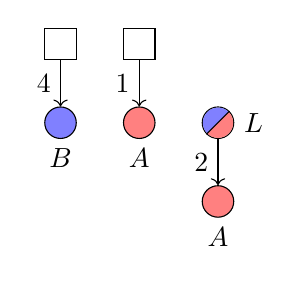
\begin{tikzpicture}[y=1cm, x=1cm]
      \node[sqadj] (a0) at (0, 0) {};
      \node[circB, label=below:$B$] (p0) at (0, -1) {};
      \draw[->] (a0) edge node[midway, left] { $4$ } (p0);

      \node[sqadj] (a2) at (1, 0) {};
      \node[circA, label=below:$A$] (pa) at (1, -1) {};
      \draw[->] (a2) edge node[midway, left] { $1$ } (pa);

      \node[circAB, label=right:$L$] (p1) at (2, -1) {};
      \node[circA, label=below:$A$] (p2) at (2, -2) {};
      \draw[->] (p1) edge node[midway, left] { $2$ } (p2);
    \end{tikzpicture}
  };

  \draw[shorten <=0.5cm, shorten >=0.3cm, -{Latex[length=2mm]}] (diag0) edge node[midway, above] {$\transfer{L}{B}{4}\; \transfer{L}{A}{1}$} (diag1);
\end{tikzpicture}
}
  \caption{
    A graphical representation of the outcome $[\allocation{B}{4}, \allocation{A}{3}]$.
    All exits are allocations, meaning
    Outcomes pay out in priority order.
    In the diagram, $B$ is drawn to the left of $A$ to show that $B$ has higher priority in the outcome of $L$.
    In this example, $L$ can afford $4$ coins for $B$, but can only afford $1$ coin for $A$.
  }\label{fig:transfer-insufficient-funds}
\end{figure}

{}\todo{This figure needs to be updated}

Allocation exits are triggered via the \textbf{transfer} operation, \transfer{A}{i}, which follows the following specification:
\begin{enumerate}
  \item Reverts if the channel $A$ is not finalized\todo{address}.
  \item Reverts if the $i$-th exit $e$ in $A$'s outcome is not an allocation.
  \item Sets $x$ to be $e.amount$.
  \item Reduces the funds held in channel $A$ by $x$. 
  \item Sends $x$ coints to $B$.
  \item Reduces $e.amount$ by $x$.
\end{enumerate} \todo{address e.amount issue}

Guarantees are triggered via the \textbf{claim} operation \claim{A}{i}\todo{decide where to fetch $x$ from}, which follows the following specification:
\begin{enumerate}
  \item Reverts if the channel $A$ is not finalized\todo{address}.
  \item Reverts if the $i$-th exit $e$ in $A$'s outcome is not a guarantee
  \item Reverts if the channel $e.target$ is not finalized.
  \item Reduces the funds held in channel $A$ by $x$. 
  \item Sends $x$ coints to the ether\todo{fill this in}
  \item Reduces $e.amount$ by $x$.
\end{enumerate} \todo{address e.amount and e.target issue}


\subsection{Recap}
\todo{Add a table outlining on-chain state transitions}
\section{Off-chain protocols}
\subsection{Ledger Channels}

A \textbf{ledger} channel is a channel which is funded directly by the ledger.

\subsubsection{Depositing into a ledger channel}
(Provide minimal explanation, and refer to the Nitro whitepaper for details.)

\subsubsection{Withdrawing from a ledger channel}

\subsection{Virtual channels}
Suppose we have peers $A = P_0, P_1, ..., P_n, P_{n+1} = B$ where:
\begin{itemize}
    \item each $(P_i, P_{i+1})$ pair already has a ledger channel $L_i$ running the consensus app
    \item Alice ($P_0$) and Bob ($P_{n+1}$) want to make (virtual) payments between each other.
\end{itemize}

We can safely fund a joint channel $J$ with the following protocol:

\textbf{Round 1}: Each participant signs a state $s$ for $J$ with $turnNum = 0$ and outcome $\{A: a_0,\; B: b_0\}$. They sign $s$ and send 

\textbf{Round 2}: For each i = 0,...,n, participants $P_i$ and $P_{i+1}$ sign an update in $L_i$ to:
\begin{itemize}
    \item deduct $a_0$ from $P_i$'s balance in $L_i$
    \item deduct $b_0$ from $P_{i+1}$'s balance in $L_i$
    \item include the allocation $G_i = {J: {amount: x, left: P_i, right: P_{i+1}}}$ where $x=a_0+b_0$
\end{itemize}


For instance, $L_i$'s outcome might change
\begin{itemize}
    \item from $[\allocation{P_i}{bal_i}, \allocation{P_{i+1}}{bal_i'}, \guarantee{X'}{x'}{foo, bar}]$
    \item to
$[\allocation{P_i}{bal_i - a_0}, \allocation{P_{i+1}}{bal_i' - b_0}, \guarantee{X'}{x'}{P_i, P_{i+1}}, \guarantee{X}{x}{P_i, P_{i+1}}].$
\end{itemize}


\textbf{Round 3}:
Alice blocks until she receives a counter-signed update in $L_0$. Bob blocks until he receives a counter-signed update in $L_n$. For $i \in \{1,\ldots,n\}$, $P_i$ blocks until they have counter-signed updates in $L_i$.

Each participant signs a post-fund state $s_1$ for $J$ with $version = 1$ and outcome $\{A: a_0, B: b_0\}$.

For each peer, the protocol is completed once a full set of signatures is received on $s_1$. At this point,
\begin{itemize}
    \item each $P_i$ has $a_0 + b_0$ fewer tokens across their two ledger channels $L_{i-1}$ and $L_i$
    \item Alice ($P_0$) has $a_0$ fewer tokens in $L_0$
    \item Bob ($P_{n+1}$) has $b_0$ fewer tokens in $L_{n}$
    \item every participant's ledger channel reductions are offset by an equal allocation to the joint channel $J$
    \item $J$'s outcome
\end{itemize}

To secure this protocol, we now specify application rules for $J$. \todo{specify}

We are now ready to state the main result of this paper:\todo{add theorem}
% \begin{theorem}
%     This protocol is secure.
% \end{theorem}

Proof: \todo{see V2 spec}

Case 1:
Case 2:
Case 3:

% \begin{cases}
%     \item{}
% \end{cases}

\subsection{Variations}

\subsubsection{Generic virtual channels.}
\todo{see the example on github}

\subsection{Reduced latency of construction.}
\todo{}

\section{Appendix}

THIS APPENDIX IS STILL A WIP.

\subsection{Overview of ForceMove}

The ForceMove protocol describes the message format and the supporting on-chain behaviour
to enable generalized, $n$-party state channels on any blockchain that supports Turing-complete, general-purpose computation.
Here we give a brief overview of the protocol to the level required to understand
the rest of the paper. For a more comprehensive explanation please refer to \cite{}.

\begin{table}[h]
  \begin{tabular}{|l|l|l|p{5cm}|}
    \hline
    \texttt{participants} & \texttt{address[]} & $P$ & The addresses used to sign updates to the channel. \\ \hline
    \texttt{nonce} & \texttt{unit256} & $k$ & Chosen to make the channel's address unique. \\ \hline
    \texttt{gameLibrary} & \texttt{address} & $L$ & The address of the gameLibrary, which defines the transition rules for this channel \\ \hline
    \texttt{challengeDuration} & \texttt{unit256} & $\eta$ & \\ \hline
    \texttt{turnNum} & \texttt{unit256} & $i$ & Increments as new states are produced. \\ \hline
    \texttt{balances} & \texttt{(address, uint256)[]} & $\beta$ & Current \textit{outcome} of the channel. \\ \hline
    \texttt{isFinal} & \texttt{bool} & $f$ & \\ \hline
    \texttt{data} & \texttt{bytes} & $\delta$ & \\ \hline
    \texttt{v} & \texttt{uint8} & &  ECDSA signature of the above arguments by the moving participant. \\ \cline{1-2}
    \texttt{r} & \texttt{bytes32} & & \\ \cline{1-2}
    \texttt{s} & \texttt{bytes32} & & \\ \hline
  \end{tabular}
  \caption{ForceMove state format}
  \label{table:force-move-state}
\end{table}

A ForceMove \textbf{state}, $\sigma_\chi^i(\beta, f, \delta)$, is specified by \textbf{turn number}, $i$,
a set of \textbf{balances}, $\beta$, a boolean flag \textbf{finalized}, $f \in \{T, F\}$, and
a chunk of unstructured \textbf{game data}, $\delta$, that will be interpreted by the game library. The
balances can be thought of as an ordered set of $(\texttt{address}, \texttt{uint256})$ pairs,
which specify how any funds allocated to the channel should be distributed if the channel 
were to finalize in the current state.

In order for a state, $\sigma_\chi^i$, to be valid it must be signed by participant, $p_j$,
where $j = i \% n$ is the remainder mod $n$. This requirement specifies that participants
in the channel must take turns when signing states.

The game library is responsible for defining a set of states and allowed transitions that
in turn define the `application' that will run inside the state channel. It does this by
defining a single boolean function, $t_L(i, \beta, \delta, \beta', \delta') \rightarrow \{ T, F\}$.
This function is used to derive an overall boolean transition function, $t$, specifying whether
a transition between two states is permitted under the rules of the protocol:
\begin{align*}
  t(\sigma_\chi^i(\beta, f, \delta), \sigma_{\chi'}^j(\beta', f', \delta') ) \Leftrightarrow &
    \chi = \chi'
    \wedge j = i + 1
    \wedge \\
    & [ (\neg f \wedge \neg f' \wedge j \leq 2n \wedge \beta = \beta' \wedge \delta = \delta') \vee \\
    & (\neg f \wedge \neg f' \wedge j > 2n \wedge t_L(n, \beta, \delta, \beta', \delta')) \vee \\
    & (f' \wedge \beta = \beta' \wedge \delta' = 0) ]
\end{align*}

In all transitions the channel properties must remain unchanged and the turn number must increment.
There are then three different modes of operation. The first mode applies in the first $2n$
states (assuming none of these are finalized) and in this mode the balances and game data
must remain unchanged. As we will see later, these states exist so that the channel can be
funded safely. We refer to the first $n$ states as the \textbf{pre-fund setup} states and
the subsequent $n$ as the \textbf{post-fund setup} states. The second mode applies to the
`normal' operation of the channel, when the game library is used to determine the allowed
transitions. The final mode concerns the finalization of the channel: at any point the current
participant can choose to exit the channel and lock in the balances in the current state.
Once this happens the only allowed transitions are to additional finalized states. Because
of this, we have no further use for the game data, $\delta$, so can remove this from the state.
Once a sequence of $n$ finalized states have been produced the channel is considered closed. We
call this sequence of $n$ finalized states a \textbf{conclusion proof}, which we will write $\bm{\sigma}^*$.



\subsection{The Consensus Game}

The Consensus Game is an important ForceMove application, which we will use heavily in the rest of the paper due to its special properties regarding outcome finalizability. In this section we introduce transition rules and explore these properties.

Like all ForceMove applications, the transition rules for the Consensus Game are specified by a game library, $L_C$, which defines the transition function, $t_{L_C}$, in terms of the turn number, $i$, the balances, $\beta$ and the game data $\delta$. $\delta = (j, x)$, where $j$ is the \textit{consensus counter} and $x$ is the \textit{proposed balances}. 
\begin{align*}
  t_{L_C}(i, \beta, (j, x), \beta', (j', x')) \Leftrightarrow
    [ & (j=n-1 \wedge j'= 0 \wedge \beta' = x = x')  \vee \\
    & (j < n-1 \wedge j' = j+1, \beta = \beta', x = x') \vee \\
    & (j'=0, \beta = \beta') ]
\end{align*}
For a given $\beta$, the consensus counter will increase from $0\dots (n-1)$ as the participants sign off on the new balances. Once all participants have signed, consensus has been reached and the channel's balances are updated.


\subsection{Proofs of Correctness}

- what do we need to prove?
- we gave the algorithms in terms of universally finalizable states.
- we now need to find the intermediate states to move betweenthem

- if we two universally finalizable states, $\sigma$, $\sigma'$
- in a consensus game channel with $n$ participants
- that are value preserving for all participants
- then it is possible to find a set of $n$ state updates that preserve value for all participants and which move from $\sigma$ and $\sigma'$

  \begin{align*}
    \sigma^{i}(\beta, (0, \beta)) & \approx [\beta]_P \\
    \sigma^{i+1}(\beta, (0, \beta')) & \approx \{\beta'\}_{p_0}[\beta]_{p_1, ..., p_{n-1}} \\
    \sigma^{i+2}(\beta, (1, \beta')) & \approx \{\beta'\}_{p_0, p_1}[\beta]_{p_2, ..., p_{n-1}} \\
    &\vdots\\
    \sigma^{i+n-1}(\beta, (n-1, \beta')) & \approx [\beta', \beta]_{p_{n-1}} \\
    \sigma^{i+n}(\beta', (0, \beta')) & \approx [\beta']_{P} \\
  \end{align*}


\subsection{Virtual Channels on Turbo}
\subsection{Payouts to Non-Participants}
\subsection{Possible Extensions}

\subsection{On-chain Operations Code}



\bibliography{main}
\bibliographystyle{ieeetr}

\end{document}
